\documentclass[11pt]{article}

    \usepackage[breakable]{tcolorbox}
    \usepackage{parskip} % Stop auto-indenting (to mimic markdown behaviour)
    

    % Basic figure setup, for now with no caption control since it's done
    % automatically by Pandoc (which extracts ![](path) syntax from Markdown).
    \usepackage{graphicx}
    % Keep aspect ratio if custom image width or height is specified
    \setkeys{Gin}{keepaspectratio}
    % Maintain compatibility with old templates. Remove in nbconvert 6.0
    \let\Oldincludegraphics\includegraphics
    % Ensure that by default, figures have no caption (until we provide a
    % proper Figure object with a Caption API and a way to capture that
    % in the conversion process - todo).
    \usepackage{caption}
    \DeclareCaptionFormat{nocaption}{}
    \captionsetup{format=nocaption,aboveskip=0pt,belowskip=0pt}

    \usepackage{float}
    \floatplacement{figure}{H} % forces figures to be placed at the correct location
    \usepackage{xcolor} % Allow colors to be defined
    \usepackage{enumerate} % Needed for markdown enumerations to work
    \usepackage{geometry} % Used to adjust the document margins
    \usepackage{amsmath} % Equations
    \usepackage{amssymb} % Equations
    \usepackage{textcomp} % defines textquotesingle
    % Hack from http://tex.stackexchange.com/a/47451/13684:
    \AtBeginDocument{%
        \def\PYZsq{\textquotesingle}% Upright quotes in Pygmentized code
    }
    \usepackage{upquote} % Upright quotes for verbatim code
    \usepackage{eurosym} % defines \euro

    \usepackage{iftex}
    \ifPDFTeX
        \usepackage[T1]{fontenc}
        \IfFileExists{alphabeta.sty}{
              \usepackage{alphabeta}
          }{
              \usepackage[mathletters]{ucs}
              \usepackage[utf8x]{inputenc}
          }
    \else
        \usepackage{fontspec}
        \usepackage{unicode-math}
    \fi

    \usepackage{fancyvrb} % verbatim replacement that allows latex
    \usepackage{grffile} % extends the file name processing of package graphics
                         % to support a larger range
    \makeatletter % fix for old versions of grffile with XeLaTeX
    \@ifpackagelater{grffile}{2019/11/01}
    {
      % Do nothing on new versions
    }
    {
      \def\Gread@@xetex#1{%
        \IfFileExists{"\Gin@base".bb}%
        {\Gread@eps{\Gin@base.bb}}%
        {\Gread@@xetex@aux#1}%
      }
    }
    \makeatother
    \usepackage[Export]{adjustbox} % Used to constrain images to a maximum size
    \adjustboxset{max size={0.9\linewidth}{0.9\paperheight}}

    % The hyperref package gives us a pdf with properly built
    % internal navigation ('pdf bookmarks' for the table of contents,
    % internal cross-reference links, web links for URLs, etc.)
    \usepackage{hyperref}
    % The default LaTeX title has an obnoxious amount of whitespace. By default,
    % titling removes some of it. It also provides customization options.
    \usepackage{titling}
    \usepackage{longtable} % longtable support required by pandoc >1.10
    \usepackage{booktabs}  % table support for pandoc > 1.12.2
    \usepackage{array}     % table support for pandoc >= 2.11.3
    \usepackage{calc}      % table minipage width calculation for pandoc >= 2.11.1
    \usepackage[inline]{enumitem} % IRkernel/repr support (it uses the enumerate* environment)
    \usepackage[normalem]{ulem} % ulem is needed to support strikethroughs (\sout)
                                % normalem makes italics be italics, not underlines
    \usepackage{soul}      % strikethrough (\st) support for pandoc >= 3.0.0
    \usepackage{mathrsfs}
    

    
    % Colors for the hyperref package
    \definecolor{urlcolor}{rgb}{0,.145,.698}
    \definecolor{linkcolor}{rgb}{.71,0.21,0.01}
    \definecolor{citecolor}{rgb}{.12,.54,.11}

    % ANSI colors
    \definecolor{ansi-black}{HTML}{3E424D}
    \definecolor{ansi-black-intense}{HTML}{282C36}
    \definecolor{ansi-red}{HTML}{E75C58}
    \definecolor{ansi-red-intense}{HTML}{B22B31}
    \definecolor{ansi-green}{HTML}{00A250}
    \definecolor{ansi-green-intense}{HTML}{007427}
    \definecolor{ansi-yellow}{HTML}{DDB62B}
    \definecolor{ansi-yellow-intense}{HTML}{B27D12}
    \definecolor{ansi-blue}{HTML}{208FFB}
    \definecolor{ansi-blue-intense}{HTML}{0065CA}
    \definecolor{ansi-magenta}{HTML}{D160C4}
    \definecolor{ansi-magenta-intense}{HTML}{A03196}
    \definecolor{ansi-cyan}{HTML}{60C6C8}
    \definecolor{ansi-cyan-intense}{HTML}{258F8F}
    \definecolor{ansi-white}{HTML}{C5C1B4}
    \definecolor{ansi-white-intense}{HTML}{A1A6B2}
    \definecolor{ansi-default-inverse-fg}{HTML}{FFFFFF}
    \definecolor{ansi-default-inverse-bg}{HTML}{000000}

    % common color for the border for error outputs.
    \definecolor{outerrorbackground}{HTML}{FFDFDF}

    % commands and environments needed by pandoc snippets
    % extracted from the output of `pandoc -s`
    \providecommand{\tightlist}{%
      \setlength{\itemsep}{0pt}\setlength{\parskip}{0pt}}
    \DefineVerbatimEnvironment{Highlighting}{Verbatim}{commandchars=\\\{\}}
    % Add ',fontsize=\small' for more characters per line
    \newenvironment{Shaded}{}{}
    \newcommand{\KeywordTok}[1]{\textcolor[rgb]{0.00,0.44,0.13}{\textbf{{#1}}}}
    \newcommand{\DataTypeTok}[1]{\textcolor[rgb]{0.56,0.13,0.00}{{#1}}}
    \newcommand{\DecValTok}[1]{\textcolor[rgb]{0.25,0.63,0.44}{{#1}}}
    \newcommand{\BaseNTok}[1]{\textcolor[rgb]{0.25,0.63,0.44}{{#1}}}
    \newcommand{\FloatTok}[1]{\textcolor[rgb]{0.25,0.63,0.44}{{#1}}}
    \newcommand{\CharTok}[1]{\textcolor[rgb]{0.25,0.44,0.63}{{#1}}}
    \newcommand{\StringTok}[1]{\textcolor[rgb]{0.25,0.44,0.63}{{#1}}}
    \newcommand{\CommentTok}[1]{\textcolor[rgb]{0.38,0.63,0.69}{\textit{{#1}}}}
    \newcommand{\OtherTok}[1]{\textcolor[rgb]{0.00,0.44,0.13}{{#1}}}
    \newcommand{\AlertTok}[1]{\textcolor[rgb]{1.00,0.00,0.00}{\textbf{{#1}}}}
    \newcommand{\FunctionTok}[1]{\textcolor[rgb]{0.02,0.16,0.49}{{#1}}}
    \newcommand{\RegionMarkerTok}[1]{{#1}}
    \newcommand{\ErrorTok}[1]{\textcolor[rgb]{1.00,0.00,0.00}{\textbf{{#1}}}}
    \newcommand{\NormalTok}[1]{{#1}}

    % Additional commands for more recent versions of Pandoc
    \newcommand{\ConstantTok}[1]{\textcolor[rgb]{0.53,0.00,0.00}{{#1}}}
    \newcommand{\SpecialCharTok}[1]{\textcolor[rgb]{0.25,0.44,0.63}{{#1}}}
    \newcommand{\VerbatimStringTok}[1]{\textcolor[rgb]{0.25,0.44,0.63}{{#1}}}
    \newcommand{\SpecialStringTok}[1]{\textcolor[rgb]{0.73,0.40,0.53}{{#1}}}
    \newcommand{\ImportTok}[1]{{#1}}
    \newcommand{\DocumentationTok}[1]{\textcolor[rgb]{0.73,0.13,0.13}{\textit{{#1}}}}
    \newcommand{\AnnotationTok}[1]{\textcolor[rgb]{0.38,0.63,0.69}{\textbf{\textit{{#1}}}}}
    \newcommand{\CommentVarTok}[1]{\textcolor[rgb]{0.38,0.63,0.69}{\textbf{\textit{{#1}}}}}
    \newcommand{\VariableTok}[1]{\textcolor[rgb]{0.10,0.09,0.49}{{#1}}}
    \newcommand{\ControlFlowTok}[1]{\textcolor[rgb]{0.00,0.44,0.13}{\textbf{{#1}}}}
    \newcommand{\OperatorTok}[1]{\textcolor[rgb]{0.40,0.40,0.40}{{#1}}}
    \newcommand{\BuiltInTok}[1]{{#1}}
    \newcommand{\ExtensionTok}[1]{{#1}}
    \newcommand{\PreprocessorTok}[1]{\textcolor[rgb]{0.74,0.48,0.00}{{#1}}}
    \newcommand{\AttributeTok}[1]{\textcolor[rgb]{0.49,0.56,0.16}{{#1}}}
    \newcommand{\InformationTok}[1]{\textcolor[rgb]{0.38,0.63,0.69}{\textbf{\textit{{#1}}}}}
    \newcommand{\WarningTok}[1]{\textcolor[rgb]{0.38,0.63,0.69}{\textbf{\textit{{#1}}}}}
    \makeatletter
    \newsavebox\pandoc@box
    \newcommand*\pandocbounded[1]{%
      \sbox\pandoc@box{#1}%
      % scaling factors for width and height
      \Gscale@div\@tempa\textheight{\dimexpr\ht\pandoc@box+\dp\pandoc@box\relax}%
      \Gscale@div\@tempb\linewidth{\wd\pandoc@box}%
      % select the smaller of both
      \ifdim\@tempb\p@<\@tempa\p@
        \let\@tempa\@tempb
      \fi
      % scaling accordingly (\@tempa < 1)
      \ifdim\@tempa\p@<\p@
        \scalebox{\@tempa}{\usebox\pandoc@box}%
      % scaling not needed, use as it is
      \else
        \usebox{\pandoc@box}%
      \fi
    }
    \makeatother

    % Define a nice break command that doesn't care if a line doesn't already
    % exist.
    \def\br{\hspace*{\fill} \\* }
    % Math Jax compatibility definitions
    \def\gt{>}
    \def\lt{<}
    \let\Oldtex\TeX
    \let\Oldlatex\LaTeX
    \renewcommand{\TeX}{\textrm{\Oldtex}}
    \renewcommand{\LaTeX}{\textrm{\Oldlatex}}
    % Document parameters
    % Document title
    \title{TP1}
    
    
    
    
    
    
    
% Pygments definitions
\makeatletter
\def\PY@reset{\let\PY@it=\relax \let\PY@bf=\relax%
    \let\PY@ul=\relax \let\PY@tc=\relax%
    \let\PY@bc=\relax \let\PY@ff=\relax}
\def\PY@tok#1{\csname PY@tok@#1\endcsname}
\def\PY@toks#1+{\ifx\relax#1\empty\else%
    \PY@tok{#1}\expandafter\PY@toks\fi}
\def\PY@do#1{\PY@bc{\PY@tc{\PY@ul{%
    \PY@it{\PY@bf{\PY@ff{#1}}}}}}}
\def\PY#1#2{\PY@reset\PY@toks#1+\relax+\PY@do{#2}}

\@namedef{PY@tok@w}{\def\PY@tc##1{\textcolor[rgb]{0.73,0.73,0.73}{##1}}}
\@namedef{PY@tok@c}{\let\PY@it=\textit\def\PY@tc##1{\textcolor[rgb]{0.24,0.48,0.48}{##1}}}
\@namedef{PY@tok@cp}{\def\PY@tc##1{\textcolor[rgb]{0.61,0.40,0.00}{##1}}}
\@namedef{PY@tok@k}{\let\PY@bf=\textbf\def\PY@tc##1{\textcolor[rgb]{0.00,0.50,0.00}{##1}}}
\@namedef{PY@tok@kp}{\def\PY@tc##1{\textcolor[rgb]{0.00,0.50,0.00}{##1}}}
\@namedef{PY@tok@kt}{\def\PY@tc##1{\textcolor[rgb]{0.69,0.00,0.25}{##1}}}
\@namedef{PY@tok@o}{\def\PY@tc##1{\textcolor[rgb]{0.40,0.40,0.40}{##1}}}
\@namedef{PY@tok@ow}{\let\PY@bf=\textbf\def\PY@tc##1{\textcolor[rgb]{0.67,0.13,1.00}{##1}}}
\@namedef{PY@tok@nb}{\def\PY@tc##1{\textcolor[rgb]{0.00,0.50,0.00}{##1}}}
\@namedef{PY@tok@nf}{\def\PY@tc##1{\textcolor[rgb]{0.00,0.00,1.00}{##1}}}
\@namedef{PY@tok@nc}{\let\PY@bf=\textbf\def\PY@tc##1{\textcolor[rgb]{0.00,0.00,1.00}{##1}}}
\@namedef{PY@tok@nn}{\let\PY@bf=\textbf\def\PY@tc##1{\textcolor[rgb]{0.00,0.00,1.00}{##1}}}
\@namedef{PY@tok@ne}{\let\PY@bf=\textbf\def\PY@tc##1{\textcolor[rgb]{0.80,0.25,0.22}{##1}}}
\@namedef{PY@tok@nv}{\def\PY@tc##1{\textcolor[rgb]{0.10,0.09,0.49}{##1}}}
\@namedef{PY@tok@no}{\def\PY@tc##1{\textcolor[rgb]{0.53,0.00,0.00}{##1}}}
\@namedef{PY@tok@nl}{\def\PY@tc##1{\textcolor[rgb]{0.46,0.46,0.00}{##1}}}
\@namedef{PY@tok@ni}{\let\PY@bf=\textbf\def\PY@tc##1{\textcolor[rgb]{0.44,0.44,0.44}{##1}}}
\@namedef{PY@tok@na}{\def\PY@tc##1{\textcolor[rgb]{0.41,0.47,0.13}{##1}}}
\@namedef{PY@tok@nt}{\let\PY@bf=\textbf\def\PY@tc##1{\textcolor[rgb]{0.00,0.50,0.00}{##1}}}
\@namedef{PY@tok@nd}{\def\PY@tc##1{\textcolor[rgb]{0.67,0.13,1.00}{##1}}}
\@namedef{PY@tok@s}{\def\PY@tc##1{\textcolor[rgb]{0.73,0.13,0.13}{##1}}}
\@namedef{PY@tok@sd}{\let\PY@it=\textit\def\PY@tc##1{\textcolor[rgb]{0.73,0.13,0.13}{##1}}}
\@namedef{PY@tok@si}{\let\PY@bf=\textbf\def\PY@tc##1{\textcolor[rgb]{0.64,0.35,0.47}{##1}}}
\@namedef{PY@tok@se}{\let\PY@bf=\textbf\def\PY@tc##1{\textcolor[rgb]{0.67,0.36,0.12}{##1}}}
\@namedef{PY@tok@sr}{\def\PY@tc##1{\textcolor[rgb]{0.64,0.35,0.47}{##1}}}
\@namedef{PY@tok@ss}{\def\PY@tc##1{\textcolor[rgb]{0.10,0.09,0.49}{##1}}}
\@namedef{PY@tok@sx}{\def\PY@tc##1{\textcolor[rgb]{0.00,0.50,0.00}{##1}}}
\@namedef{PY@tok@m}{\def\PY@tc##1{\textcolor[rgb]{0.40,0.40,0.40}{##1}}}
\@namedef{PY@tok@gh}{\let\PY@bf=\textbf\def\PY@tc##1{\textcolor[rgb]{0.00,0.00,0.50}{##1}}}
\@namedef{PY@tok@gu}{\let\PY@bf=\textbf\def\PY@tc##1{\textcolor[rgb]{0.50,0.00,0.50}{##1}}}
\@namedef{PY@tok@gd}{\def\PY@tc##1{\textcolor[rgb]{0.63,0.00,0.00}{##1}}}
\@namedef{PY@tok@gi}{\def\PY@tc##1{\textcolor[rgb]{0.00,0.52,0.00}{##1}}}
\@namedef{PY@tok@gr}{\def\PY@tc##1{\textcolor[rgb]{0.89,0.00,0.00}{##1}}}
\@namedef{PY@tok@ge}{\let\PY@it=\textit}
\@namedef{PY@tok@gs}{\let\PY@bf=\textbf}
\@namedef{PY@tok@ges}{\let\PY@bf=\textbf\let\PY@it=\textit}
\@namedef{PY@tok@gp}{\let\PY@bf=\textbf\def\PY@tc##1{\textcolor[rgb]{0.00,0.00,0.50}{##1}}}
\@namedef{PY@tok@go}{\def\PY@tc##1{\textcolor[rgb]{0.44,0.44,0.44}{##1}}}
\@namedef{PY@tok@gt}{\def\PY@tc##1{\textcolor[rgb]{0.00,0.27,0.87}{##1}}}
\@namedef{PY@tok@err}{\def\PY@bc##1{{\setlength{\fboxsep}{\string -\fboxrule}\fcolorbox[rgb]{1.00,0.00,0.00}{1,1,1}{\strut ##1}}}}
\@namedef{PY@tok@kc}{\let\PY@bf=\textbf\def\PY@tc##1{\textcolor[rgb]{0.00,0.50,0.00}{##1}}}
\@namedef{PY@tok@kd}{\let\PY@bf=\textbf\def\PY@tc##1{\textcolor[rgb]{0.00,0.50,0.00}{##1}}}
\@namedef{PY@tok@kn}{\let\PY@bf=\textbf\def\PY@tc##1{\textcolor[rgb]{0.00,0.50,0.00}{##1}}}
\@namedef{PY@tok@kr}{\let\PY@bf=\textbf\def\PY@tc##1{\textcolor[rgb]{0.00,0.50,0.00}{##1}}}
\@namedef{PY@tok@bp}{\def\PY@tc##1{\textcolor[rgb]{0.00,0.50,0.00}{##1}}}
\@namedef{PY@tok@fm}{\def\PY@tc##1{\textcolor[rgb]{0.00,0.00,1.00}{##1}}}
\@namedef{PY@tok@vc}{\def\PY@tc##1{\textcolor[rgb]{0.10,0.09,0.49}{##1}}}
\@namedef{PY@tok@vg}{\def\PY@tc##1{\textcolor[rgb]{0.10,0.09,0.49}{##1}}}
\@namedef{PY@tok@vi}{\def\PY@tc##1{\textcolor[rgb]{0.10,0.09,0.49}{##1}}}
\@namedef{PY@tok@vm}{\def\PY@tc##1{\textcolor[rgb]{0.10,0.09,0.49}{##1}}}
\@namedef{PY@tok@sa}{\def\PY@tc##1{\textcolor[rgb]{0.73,0.13,0.13}{##1}}}
\@namedef{PY@tok@sb}{\def\PY@tc##1{\textcolor[rgb]{0.73,0.13,0.13}{##1}}}
\@namedef{PY@tok@sc}{\def\PY@tc##1{\textcolor[rgb]{0.73,0.13,0.13}{##1}}}
\@namedef{PY@tok@dl}{\def\PY@tc##1{\textcolor[rgb]{0.73,0.13,0.13}{##1}}}
\@namedef{PY@tok@s2}{\def\PY@tc##1{\textcolor[rgb]{0.73,0.13,0.13}{##1}}}
\@namedef{PY@tok@sh}{\def\PY@tc##1{\textcolor[rgb]{0.73,0.13,0.13}{##1}}}
\@namedef{PY@tok@s1}{\def\PY@tc##1{\textcolor[rgb]{0.73,0.13,0.13}{##1}}}
\@namedef{PY@tok@mb}{\def\PY@tc##1{\textcolor[rgb]{0.40,0.40,0.40}{##1}}}
\@namedef{PY@tok@mf}{\def\PY@tc##1{\textcolor[rgb]{0.40,0.40,0.40}{##1}}}
\@namedef{PY@tok@mh}{\def\PY@tc##1{\textcolor[rgb]{0.40,0.40,0.40}{##1}}}
\@namedef{PY@tok@mi}{\def\PY@tc##1{\textcolor[rgb]{0.40,0.40,0.40}{##1}}}
\@namedef{PY@tok@il}{\def\PY@tc##1{\textcolor[rgb]{0.40,0.40,0.40}{##1}}}
\@namedef{PY@tok@mo}{\def\PY@tc##1{\textcolor[rgb]{0.40,0.40,0.40}{##1}}}
\@namedef{PY@tok@ch}{\let\PY@it=\textit\def\PY@tc##1{\textcolor[rgb]{0.24,0.48,0.48}{##1}}}
\@namedef{PY@tok@cm}{\let\PY@it=\textit\def\PY@tc##1{\textcolor[rgb]{0.24,0.48,0.48}{##1}}}
\@namedef{PY@tok@cpf}{\let\PY@it=\textit\def\PY@tc##1{\textcolor[rgb]{0.24,0.48,0.48}{##1}}}
\@namedef{PY@tok@c1}{\let\PY@it=\textit\def\PY@tc##1{\textcolor[rgb]{0.24,0.48,0.48}{##1}}}
\@namedef{PY@tok@cs}{\let\PY@it=\textit\def\PY@tc##1{\textcolor[rgb]{0.24,0.48,0.48}{##1}}}

\def\PYZbs{\char`\\}
\def\PYZus{\char`\_}
\def\PYZob{\char`\{}
\def\PYZcb{\char`\}}
\def\PYZca{\char`\^}
\def\PYZam{\char`\&}
\def\PYZlt{\char`\<}
\def\PYZgt{\char`\>}
\def\PYZsh{\char`\#}
\def\PYZpc{\char`\%}
\def\PYZdl{\char`\$}
\def\PYZhy{\char`\-}
\def\PYZsq{\char`\'}
\def\PYZdq{\char`\"}
\def\PYZti{\char`\~}
% for compatibility with earlier versions
\def\PYZat{@}
\def\PYZlb{[}
\def\PYZrb{]}
\makeatother


    % For linebreaks inside Verbatim environment from package fancyvrb.
    \makeatletter
        \newbox\Wrappedcontinuationbox
        \newbox\Wrappedvisiblespacebox
        \newcommand*\Wrappedvisiblespace {\textcolor{red}{\textvisiblespace}}
        \newcommand*\Wrappedcontinuationsymbol {\textcolor{red}{\llap{\tiny$\m@th\hookrightarrow$}}}
        \newcommand*\Wrappedcontinuationindent {3ex }
        \newcommand*\Wrappedafterbreak {\kern\Wrappedcontinuationindent\copy\Wrappedcontinuationbox}
        % Take advantage of the already applied Pygments mark-up to insert
        % potential linebreaks for TeX processing.
        %        {, <, #, %, $, ' and ": go to next line.
        %        _, }, ^, &, >, - and ~: stay at end of broken line.
        % Use of \textquotesingle for straight quote.
        \newcommand*\Wrappedbreaksatspecials {%
            \def\PYGZus{\discretionary{\char`\_}{\Wrappedafterbreak}{\char`\_}}%
            \def\PYGZob{\discretionary{}{\Wrappedafterbreak\char`\{}{\char`\{}}%
            \def\PYGZcb{\discretionary{\char`\}}{\Wrappedafterbreak}{\char`\}}}%
            \def\PYGZca{\discretionary{\char`\^}{\Wrappedafterbreak}{\char`\^}}%
            \def\PYGZam{\discretionary{\char`\&}{\Wrappedafterbreak}{\char`\&}}%
            \def\PYGZlt{\discretionary{}{\Wrappedafterbreak\char`\<}{\char`\<}}%
            \def\PYGZgt{\discretionary{\char`\>}{\Wrappedafterbreak}{\char`\>}}%
            \def\PYGZsh{\discretionary{}{\Wrappedafterbreak\char`\#}{\char`\#}}%
            \def\PYGZpc{\discretionary{}{\Wrappedafterbreak\char`\%}{\char`\%}}%
            \def\PYGZdl{\discretionary{}{\Wrappedafterbreak\char`\$}{\char`\$}}%
            \def\PYGZhy{\discretionary{\char`\-}{\Wrappedafterbreak}{\char`\-}}%
            \def\PYGZsq{\discretionary{}{\Wrappedafterbreak\textquotesingle}{\textquotesingle}}%
            \def\PYGZdq{\discretionary{}{\Wrappedafterbreak\char`\"}{\char`\"}}%
            \def\PYGZti{\discretionary{\char`\~}{\Wrappedafterbreak}{\char`\~}}%
        }
        % Some characters . , ; ? ! / are not pygmentized.
        % This macro makes them "active" and they will insert potential linebreaks
        \newcommand*\Wrappedbreaksatpunct {%
            \lccode`\~`\.\lowercase{\def~}{\discretionary{\hbox{\char`\.}}{\Wrappedafterbreak}{\hbox{\char`\.}}}%
            \lccode`\~`\,\lowercase{\def~}{\discretionary{\hbox{\char`\,}}{\Wrappedafterbreak}{\hbox{\char`\,}}}%
            \lccode`\~`\;\lowercase{\def~}{\discretionary{\hbox{\char`\;}}{\Wrappedafterbreak}{\hbox{\char`\;}}}%
            \lccode`\~`\:\lowercase{\def~}{\discretionary{\hbox{\char`\:}}{\Wrappedafterbreak}{\hbox{\char`\:}}}%
            \lccode`\~`\?\lowercase{\def~}{\discretionary{\hbox{\char`\?}}{\Wrappedafterbreak}{\hbox{\char`\?}}}%
            \lccode`\~`\!\lowercase{\def~}{\discretionary{\hbox{\char`\!}}{\Wrappedafterbreak}{\hbox{\char`\!}}}%
            \lccode`\~`\/\lowercase{\def~}{\discretionary{\hbox{\char`\/}}{\Wrappedafterbreak}{\hbox{\char`\/}}}%
            \catcode`\.\active
            \catcode`\,\active
            \catcode`\;\active
            \catcode`\:\active
            \catcode`\?\active
            \catcode`\!\active
            \catcode`\/\active
            \lccode`\~`\~
        }
    \makeatother

    \let\OriginalVerbatim=\Verbatim
    \makeatletter
    \renewcommand{\Verbatim}[1][1]{%
        %\parskip\z@skip
        \sbox\Wrappedcontinuationbox {\Wrappedcontinuationsymbol}%
        \sbox\Wrappedvisiblespacebox {\FV@SetupFont\Wrappedvisiblespace}%
        \def\FancyVerbFormatLine ##1{\hsize\linewidth
            \vtop{\raggedright\hyphenpenalty\z@\exhyphenpenalty\z@
                \doublehyphendemerits\z@\finalhyphendemerits\z@
                \strut ##1\strut}%
        }%
        % If the linebreak is at a space, the latter will be displayed as visible
        % space at end of first line, and a continuation symbol starts next line.
        % Stretch/shrink are however usually zero for typewriter font.
        \def\FV@Space {%
            \nobreak\hskip\z@ plus\fontdimen3\font minus\fontdimen4\font
            \discretionary{\copy\Wrappedvisiblespacebox}{\Wrappedafterbreak}
            {\kern\fontdimen2\font}%
        }%

        % Allow breaks at special characters using \PYG... macros.
        \Wrappedbreaksatspecials
        % Breaks at punctuation characters . , ; ? ! and / need catcode=\active
        \OriginalVerbatim[#1,codes*=\Wrappedbreaksatpunct]%
    }
    \makeatother

    % Exact colors from NB
    \definecolor{incolor}{HTML}{303F9F}
    \definecolor{outcolor}{HTML}{D84315}
    \definecolor{cellborder}{HTML}{CFCFCF}
    \definecolor{cellbackground}{HTML}{F7F7F7}

    % prompt
    \makeatletter
    \newcommand{\boxspacing}{\kern\kvtcb@left@rule\kern\kvtcb@boxsep}
    \makeatother
    \newcommand{\prompt}[4]{
        {\ttfamily\llap{{\color{#2}[#3]:\hspace{3pt}#4}}\vspace{-\baselineskip}}
    }
    

    
    % Prevent overflowing lines due to hard-to-break entities
    \sloppy
    % Setup hyperref package
    \hypersetup{
      breaklinks=true,  % so long urls are correctly broken across lines
      colorlinks=true,
      urlcolor=urlcolor,
      linkcolor=linkcolor,
      citecolor=citecolor,
      }
    % Slightly bigger margins than the latex defaults
    
    \geometry{verbose,tmargin=1in,bmargin=1in,lmargin=1in,rmargin=1in}
    
    

\usepackage{fancyhdr} % Para encabezado/pie
\usepackage{lastpage} % Para número total de páginas
\pagestyle{fancy}

% Encabezado
\fancyhead[L]{\textbf{Inteligencia Aritificial - Trabajo Práctico 1}}
\fancyhead[C]{}
\fancyhead[R]{Grupo 2}

% Pie de página
\fancyfoot[L]{}
\fancyfoot[C]{}
\fancyfoot[R]{Página \thepage\ de \pageref{LastPage}}


\begin{document}
    
    \maketitle
    
    

    
    \section*{Temas Tratados en el Trabajo Práctico
1}\label{temas-tratados-en-el-trabajo-pruxe1ctico-1}

\begin{itemize}
\item
  Diferencia entre Inteligencia e Inteligencia Artificial.
\item
  Concepto de omnisciencia, aprendizaje y autonomía.
\item
  Definición de Agente y sus características. Clasificación de Agentes
  según su estructura.
\item
  Identificación y categorización del Entorno de Trabajo en tabla REAS.
\item
  Caracterización del Entorno de Trabajo.
\end{itemize}

\section{Anotaciones}\label{anotaciones}

``Acordarse de la definición de agente''

    \section{Ejercicios Teóricos}\label{ejercicios-teuxf3ricos}

\subsubsection{1. Defina con sus propias palabras inteligencia natural,
inteligencia artificial y
agente.}\label{defina-con-sus-propias-palabras-inteligencia-natural-inteligencia-artificial-y-agente.}

    \begin{itemize}
\item
  Inteligencia natural: Es la inteligencia que tiene naturalmente el ser
  humano, animales y seres vivos las cuales son otorgadas por la
  naturaleza y nos da la capacidad de aprender, razonar, resolver
  problemas y adaptarnos a nuestro entorno.
\item
  Inteligencia artificial: Es la inteligencia desarrollada en maquinas o
  programas las cuales pueden realizar tareas que normalmente requieren
  ser realizadas por humanos, estos son capaces de aprender, razonar y
  adaptarse al entorno.
\item
  Agente: Es una entidad natural o artificial que percibe su entorno y
  actua de manera autonoma para lograr el resultado para el que fue
  creado.
\end{itemize}

    \subsubsection{2. ¿Qué es un agente
racional?}\label{quuxe9-es-un-agente-racional}

    \begin{itemize}
\tightlist
\item
  Un agente racional es una entidad que percibe su entorno y actua de
  manera que maximiza su rendimiento utilizando los sensores que posee
  para tomar las decisiones mas optimas.
\end{itemize}

    \subsubsection{3. ¿Un agente es siempre una
computadora?}\label{un-agente-es-siempre-una-computadora}

    \begin{itemize}
\tightlist
\item
  No, un agente no siempre es una computadora existen tambien agentes
  organicos como proteinas creadas para combatir enfermedades o agentes
  mecanicos muy simples como el ejemplo del apagador de velas.
\end{itemize}

    \subsubsection{4. Defina Omnisciencia, Aprendizaje y
Autonomía.}\label{defina-omnisciencia-aprendizaje-y-autonomuxeda.}

    \begin{itemize}
\item
  Omnisciencia: Es la capacidad de un agente de conocer el estado actual
  completo de su entorno en todo momento, es aquel que tiene acceso a
  toda la informacion del entorno a pesar de que pueda cumplir con su
  tarea sin toda esa infromacion.
\item
  Aprendizaje: Es la capacidad de un agente de mejorar su rendimiento y
  adaptar sus acciones a lo largo del tiempo, lo cual hace que pueda
  modificar sus decisiones basandose en experiencias previas.
\item
  Autonomia: Es la capacidad de un agente de operar independientemente
  sin la intervencion o control humano directo, tomando sus propias
  decisiones y acciones.
\end{itemize}

    \subsubsection{\texorpdfstring{5. Defina cada tipo de agente en función
de su \textbf{estructura} y dé un ejemplo de cada
categoría.}{5. Defina cada tipo de agente en función de su estructura y dé un ejemplo de cada categoría.}}\label{defina-cada-tipo-de-agente-en-funciuxf3n-de-su-estructura-y-duxe9-un-ejemplo-de-cada-categoruxeda.}

    Las diferentes estructuras que podemos modelar para los agentes son:

\begin{itemize}
\item
  Agente Reactivo Simple:

  El agente reactivo simple, como su nombre lo indica, es una estructura
  primitiva que funciona de manera sencilla: el sensor toma lecturas del
  entorno, analiza ``¿cómo es el mundo ahora?'' y con esa información,
  junto con las ``reglas de condición-acción'' con las que fue creado,
  define que acción debe tomar para modificar el entorno y realiza la
  acción mediante actuadores.

  Un ejemplo de este tipo de agentes es una pava eléctrica, que al
  pulsar un botón empieza a calentar el agua hasta que el bimetálico
  alcance una cierta temperatura, independientemente de si tiene agua u
  otro líquido, o de si ya se calentó el líquido previamente.
\item
  Agente Reactivo Basado en Modelos

  El agente reactivo basado en modelos tambíen cuenta con sensores que
  permite leer cúal es el estado del entorno actual, pero la información
  obtenida es almacenada y utilizada para mantener un seguimiento del
  entorno que no es evidente con la percepción instante a instante.
  Teniendo en cuenta tanto el modelo del entorno como los parámetros
  sensados, se refiere a las reglas ``condición-acción'', se determina
  que acción tomar y finalmente se acciona con los actuadores.

  Un ejemplo de este tipo de agentes es un robot que solo se mueve en un
  plano euclidiano: debe ir del punto A al punto B, y con trigonometría
  (modelo matemático) se calcula la ruta en linea recta.
\item
  Agente Basados en Objetivos

  El agente basado en objetivos agrega con respecto al agente basado en
  modelos un bloque que analiza las acciones posibles y elije cualquier
  acción que permita llegar a una meta predeterminada.

  Un ejemplo de este tipo de agentes es un robot que solo se mueve en un
  plano euclidiano (como el ejemplo anterior) pero que es capaz de
  distinguir si hay un obstaculo e idear un camino (no necesariamente
  recto) que permita ir desde el punto A hasta el punto B (sea cual sea
  la ruta que se elija).
\item
  Agente Basado en Utilidad

  El agente basado en utilidad agrega respecto al agente basado en
  utilidades un bloque de ``utilidad'' o ``eficiencia''. Esto quiere
  decir que, de entre todas las acciones posibles que me permitan llegar
  a mi meta, se tomará la acción que sea más ``efectiva'' (respecto a un
  parámetro de ``comodidad'').

  Un ejemplo de este tipo de agentes es el sistema de temperatura
  inteligente de un edificio, que busca ajustar la temperatura y la
  ventilación con la idea de maximizar el confort y minimizar el gasto
  energético simultaneamente.
\item
  Agentes que Aprenden

  El agente que aprende agrega respecto al agente basado en utilidad una
  capacidad de mejorar sus comportamiento con el paso del tiempo a
  partir de la experiencia. Tiene bloques de ``Elemento de aprendizaje''
  y otro de ``Generador de Problemas'' así como realimentación. Es capaz
  de provar diferentes métodos y calibrar la mejor ruta de acción.

  Un ejemplo de este tipo de agentes es un software de hospital, que
  basado en datos de miles de pacientes genera un diagnóstico para una
  persona particular a partir de los datos de salud de la misma.
\end{itemize}

    \subsubsection{\texorpdfstring{6. Para los siguientes entornos de
trabajo indique sus
\textbf{propiedades}:}{6. Para los siguientes entornos de trabajo indique sus propiedades:}}\label{para-los-siguientes-entornos-de-trabajo-indique-sus-propiedades}

\begin{verbatim}
    a. Una partida de ajedrez.
\end{verbatim}

\begin{longtable}[]{@{}
  >{\raggedright\arraybackslash}p{(\linewidth - 2\tabcolsep) * \real{0.0684}}
  >{\raggedright\arraybackslash}p{(\linewidth - 2\tabcolsep) * \real{0.9316}}@{}}
\toprule\noalign{}
\begin{minipage}[b]{\linewidth}\raggedright
Propiedades
\end{minipage} & \begin{minipage}[b]{\linewidth}\raggedright
\end{minipage} \\
\midrule\noalign{}
\endhead
\bottomrule\noalign{}
\endlastfoot
Observabilidad & Total. Se pueden ver el estado de todas las piezas del
tablero. \\
Determinista/Estocástico & Estocástico. El ajedrez tiene \(10^{150}\)
posibles combinaciones entre todas las piezas, por lo que cada jugada es
un evento probabilístico. \\
Episódico/Secuencial & Secuencial. Ambos jugadores mantienen un
historial de los movimientos propios y los del oponente, por lo que cada
decisión previa afecta la toma de decisiones futuras. Aunque es posible
que un jugador continúe una partida de ajedrez ya iniciada sin necesidad
de tener una lista de todos los movimientos previos de ambos bandos. \\
Estático/Dinámico & Estático. Durante el turno de un jugador, el
contrincante no puede mover una de sus piezas. \\
Discreto/Contínuo & Discreto. Cada pieza tiene un número concreto de
movimientos cada una, las cuales son claramente definidas. \\
Agente & Multiagente. Existen 2 agentes: cada jugador. \\
\end{longtable}

\begin{verbatim}
    b. Un partido de baloncesto.
\end{verbatim}

\begin{longtable}[]{@{}
  >{\raggedright\arraybackslash}p{(\linewidth - 2\tabcolsep) * \real{0.0769}}
  >{\raggedright\arraybackslash}p{(\linewidth - 2\tabcolsep) * \real{0.9231}}@{}}
\toprule\noalign{}
\begin{minipage}[b]{\linewidth}\raggedright
Propiedades
\end{minipage} & \begin{minipage}[b]{\linewidth}\raggedright
\end{minipage} \\
\midrule\noalign{}
\endhead
\bottomrule\noalign{}
\endlastfoot
Observabilidad & Total. Un jugador puede ver a todos sus compañeros y
contrincantes, la posición del balón y el puntaje de cada equipo. \\
Determinista/Estocástico & Estocástico. El partido de baloncesto depende
de las jugadas de cada equipo y adicionalmente de las acciones
individuales que tome cada jugador. No es posible determinar como se
desarrollara un juego en su plenitud (a lo sumo se podrá adivinar una de
las muchas jugadas del contrincante). \\
Episódico/Secuencial & Secuencial. Si un jugador corre mucho, se cansará
rápido, por lo que sus acciones pasadas afectan las decisiones
futuras. \\
Estático/Dinámico & Dinámico. Ambos equipos pueden responder o modificar
su jugada mientras el contraincante planea una estrategia. \\
Discreto/Contínuo & Continuo. La posición de cada jugador es una
variable continua, aunque puede discretizarse en zonas. \\
Agente & Multiajentes. Son 10 jugadores en la cancha (y jugadores
adicionales en la banca). \\
\end{longtable}

\begin{verbatim}
    c. El juego Pacman.
\end{verbatim}

\begin{longtable}[]{@{}
  >{\raggedright\arraybackslash}p{(\linewidth - 2\tabcolsep) * \real{0.1283}}
  >{\raggedright\arraybackslash}p{(\linewidth - 2\tabcolsep) * \real{0.8717}}@{}}
\toprule\noalign{}
\begin{minipage}[b]{\linewidth}\raggedright
Propiedades
\end{minipage} & \begin{minipage}[b]{\linewidth}\raggedright
\end{minipage} \\
\midrule\noalign{}
\endhead
\bottomrule\noalign{}
\endlastfoot
Observabilidad & Total. Conozco la posición de todos los personajes y
objetos. \\
Determinista/Estocástico & Determinista. Es un juego basado en un código
informático, se tienen estrategias comprobadas para jugar, donde una
acción determinada produce una respuesta acorde. \\
Episódico/Secuencial & Secuencial. Si ya se comió todos los ``puntos''
de un segmento, este hecho afectará mi juicio a la hora de decidir si ir
o no por ese camino. \\
Estático/Dinámico & Dinámico. Los ``fantasmitas'' te persiguen incluso
cuando planeas en qué dirección ir. \\
Discreto/Contínuo & Discreto. Cada acción esta acotada (``Frame Per
Second''). \\
Agente & Individual. El único agente es el jugador. \\
\end{longtable}

\begin{verbatim}
    d. El truco.
\end{verbatim}

\begin{longtable}[]{@{}
  >{\raggedright\arraybackslash}p{(\linewidth - 2\tabcolsep) * \real{0.0980}}
  >{\raggedright\arraybackslash}p{(\linewidth - 2\tabcolsep) * \real{0.9020}}@{}}
\toprule\noalign{}
\begin{minipage}[b]{\linewidth}\raggedright
Propiedades
\end{minipage} & \begin{minipage}[b]{\linewidth}\raggedright
\end{minipage} \\
\midrule\noalign{}
\endhead
\bottomrule\noalign{}
\endlastfoot
Observabilidad & Parcial. No conozco las cartas de nadie excepto las
mias. \\
Determinista/Estocástico & Estocástico. Existen probabilidades de que
toquen una mano específica, por lo que es un juego de azar. \\
Episódico/Secuencial & Episódico. Cada nueva mano no depende de las
acciones de la mano anterior. Aunque el puntaje total del juego puede
condicionar mi estrategia de juego (es decir, si voy perdiendo estaré
condicionado a jugar más agresivo). \\
Estático/Dinámico & Estático. Es un juego por turnos. \\
Discreto/Contínuo & Discreto. Las acciones posibles estan acotadas. \\
Agente & Multiagente. Existen al menos 2 (o máximo 6) jugadores. \\
\end{longtable}

\begin{verbatim}
    e. Las damas.
\end{verbatim}

\begin{longtable}[]{@{}
  >{\raggedright\arraybackslash}p{(\linewidth - 2\tabcolsep) * \real{0.0684}}
  >{\raggedright\arraybackslash}p{(\linewidth - 2\tabcolsep) * \real{0.9316}}@{}}
\toprule\noalign{}
\begin{minipage}[b]{\linewidth}\raggedright
Propiedades
\end{minipage} & \begin{minipage}[b]{\linewidth}\raggedright
\end{minipage} \\
\midrule\noalign{}
\endhead
\bottomrule\noalign{}
\endlastfoot
Observabilidad & Total. Puedo ver la posición de todas las fichas en el
tablero. \\
Determinista/Estocástico & Estocástico. Si bien menos que en el ajedrez,
en el juego existen más de \(10^{20}\) posiciones posibles. \\
Episódico/Secuencial & Secuencial. Ambos jugadores mantienen un
historial de los movimientos propios y los del oponente, por lo que cada
decisión previa afecta la toma de decisiones futuras. Aunque es posible
que un jugador continúe una partida de damas ya iniciada sin necesidad
de tener una lista de todos los movimientos previos de ambos bandos. \\
Estático/Dinámico & Estático. Durante el turno de un jugador, el
contrincante no puede mover una de sus piezas. \\
Discreto/Contínuo & Discreto. Cada pieza tiene un número concreto de
movimientos cada una, las cuales son claramente definidas. \\
Agente & Multiagente. Existen 2 agentes: cada jugador. \\
\end{longtable}

\begin{verbatim}
    f. El juego tres en raya.
\end{verbatim}

\begin{longtable}[]{@{}
  >{\raggedright\arraybackslash}p{(\linewidth - 2\tabcolsep) * \real{0.1304}}
  >{\raggedright\arraybackslash}p{(\linewidth - 2\tabcolsep) * \real{0.8696}}@{}}
\toprule\noalign{}
\begin{minipage}[b]{\linewidth}\raggedright
Propiedades
\end{minipage} & \begin{minipage}[b]{\linewidth}\raggedright
\end{minipage} \\
\midrule\noalign{}
\endhead
\bottomrule\noalign{}
\endlastfoot
Observabilidad & Total. Puedo ver la posición de todas las fichas en el
tablero. \\
Determinista/Estocástico & Estocástico. Si bien menos que en el ajedrez,
en el juego existen \(9!\) posiciones posibles. \\
Episódico/Secuencial & Episódico. En el sentido de que cada partida
nueva es independiente del resultado de la partida anterior
(considerando al juego como ``un conjunto de partidas''). \\
Estático/Dinámico & Estático. Durante el turno de un jugador, el
contrincante no puede mover una de sus piezas. \\
Discreto/Contínuo & Discreto. Existe un número finito de acciones. \\
Agente & Multiagente. Existen 2 agentes: cada jugador. \\
\end{longtable}

\begin{verbatim}
    g. Un jugador de Pokémon Go.
\end{verbatim}

\begin{longtable}[]{@{}
  >{\raggedright\arraybackslash}p{(\linewidth - 2\tabcolsep) * \real{0.1171}}
  >{\raggedright\arraybackslash}p{(\linewidth - 2\tabcolsep) * \real{0.8829}}@{}}
\toprule\noalign{}
\begin{minipage}[b]{\linewidth}\raggedright
Propiedades
\end{minipage} & \begin{minipage}[b]{\linewidth}\raggedright
\end{minipage} \\
\midrule\noalign{}
\endhead
\bottomrule\noalign{}
\endlastfoot
Observabilidad & Parcial. El jugador no sabe la posición de casi ningún
``pokemon'' (criatura), a menos que este en la inmidiatez. \\
Determinista/Estocástico & Estocástico. No se sabe la posición exacta de
ningún pokemon (por más de que el código del juego lo maneje de forma
deterministica, a efectos prácticos el evento es probabilístico). \\
Episódico/Secuencial & Episódico. En el sentido de ``atrapar
criaturas'', atrapar una criatura A no me determina si atraparé una
criatura B ó C. \\
Estático/Dinámico & Dinámico. Los pokemons pueden aparecer y desaparecer
mientras me acerco a atraparlos. \\
Discreto/Contínuo & Continuo. La posición de tanto el jugador como de
los ``pokemons'' se distribuye de manera continua en toda la localidad
(mapa). \\
Agente & Individual. A lo que ``atrapar pokemons'' respecta, el agente
es único: el jugador. \\
\end{longtable}

\begin{verbatim}
    h. Un robot explorador autónomo de Marte.
\end{verbatim}

\begin{longtable}[]{@{}
  >{\raggedright\arraybackslash}p{(\linewidth - 2\tabcolsep) * \real{0.1622}}
  >{\raggedright\arraybackslash}p{(\linewidth - 2\tabcolsep) * \real{0.8378}}@{}}
\toprule\noalign{}
\begin{minipage}[b]{\linewidth}\raggedright
Propiedades
\end{minipage} & \begin{minipage}[b]{\linewidth}\raggedright
\end{minipage} \\
\midrule\noalign{}
\endhead
\bottomrule\noalign{}
\endlastfoot
Observabilidad & Parcial. El robot no conoce la totalidad del
planeta. \\
Determinista/Estocástico & Estocástico \\
Episódico/Secuencial & Secuencial. Si el robot se desplaza muy rápido y
se daña, este evento tendrá importancia para la toma de decisiones
futuras. \\
Estático/Dinámico & Dinámico. A medida que el robot se mueve, el clima
del planeta podría modificarse constantemente. \\
Discreto/Contínuo & Continuo. La posición del robot se debe determinar,
y dicha coordenada se considera ``continua''. \\
Agente & Individual. Solo el robot acciona e interactúa con el entorno
(al ser autónomo). \\
\end{longtable}

    \subsubsection{7. Elabore una tabla REAS para los siguientes entornos de
trabajo:}\label{elabore-una-tabla-reas-para-los-siguientes-entornos-de-trabajo}

\begin{verbatim}
    a. Crucigrama.

    b. Taxi circulando.

    c. Robot clasificador de piezas.
\end{verbatim}

    \begin{longtable}[]{@{}
  >{\raggedright\arraybackslash}p{(\linewidth - 10\tabcolsep) * \real{0.2597}}
  >{\raggedright\arraybackslash}p{(\linewidth - 10\tabcolsep) * \real{0.1688}}
  >{\raggedright\arraybackslash}p{(\linewidth - 10\tabcolsep) * \real{0.1688}}
  >{\raggedright\arraybackslash}p{(\linewidth - 10\tabcolsep) * \real{0.1169}}
  >{\raggedright\arraybackslash}p{(\linewidth - 10\tabcolsep) * \real{0.1558}}
  >{\raggedright\arraybackslash}p{(\linewidth - 10\tabcolsep) * \real{0.1299}}@{}}
\toprule\noalign{}
\begin{minipage}[b]{\linewidth}\raggedright
Entorno de trabajo
\end{minipage} & \begin{minipage}[b]{\linewidth}\raggedright
Descripcion
\end{minipage} & \begin{minipage}[b]{\linewidth}\raggedright
Rendimiento
\end{minipage} & \begin{minipage}[b]{\linewidth}\raggedright
Entorno
\end{minipage} & \begin{minipage}[b]{\linewidth}\raggedright
Actuadores
\end{minipage} & \begin{minipage}[b]{\linewidth}\raggedright
Sensores
\end{minipage} \\
\midrule\noalign{}
\endhead
\bottomrule\noalign{}
\endlastfoot
Crucigrama & Se plantea un crucigrama con una serie de pistas para que
resuelva una persona. & Crucigrama resuelto de forma correcta (que
coincida con la solución). & Ambiente iluminado, lapicera, persona que
resuelve el crucigrama. & Inteligencia de la persona y su capacidad de
escribir. & Vista de la Persona. \\
Taxi & Taxi conducido por una persona. & Transportar a los pasajeros a
su destino de forma segura y en un tiempo prudencial. & Calles,
vehículos, peatones, señales de tránsito. & Motor, dirección, frenos,
acelerador, caja de cambios accionados por el conductor. & Velocímetro,
GPS, espejos retrovisores y vista del conductor. \\
Robot clasificador de piezas & Brazo robot de 6 grados de libertad con
una pinza como efector final que le permite agarrar piezas que vienen en
una cinta transportadora, identificarlas y colocarlas en su lugar según
algún criterio. & Que los tipos de piezas resulten correctamente
clasificadas según un parámetro indicado, sin errores y lo más rápido
posible. & Cinta transportadora en movimiento, piezas, recipientes para
depositar las piezas. & Servomotores de los ejes del brazo robot,
pinzas. & Cámara o sensor de visión artificial, sensores de proximidad y
de movimiento. \\
\end{longtable}

    \section{Ejercicios Prácticos}\label{ejercicios-pruxe1cticos}

\subsubsection{8. La Hormiga de Langton es un agente capaz de modificar
el estado de la casilla en la que se encuentra para colorearla o bien de
blanco o de negro. Al comenzar, la ubicación de la hormiga es una
casilla aleatoria y mira hacia una de las cuatro casillas adyacentes.
Si\ldots{}}\label{la-hormiga-de-langton-es-un-agente-capaz-de-modificar-el-estado-de-la-casilla-en-la-que-se-encuentra-para-colorearla-o-bien-de-blanco-o-de-negro.-al-comenzar-la-ubicaciuxf3n-de-la-hormiga-es-una-casilla-aleatoria-y-mira-hacia-una-de-las-cuatro-casillas-adyacentes.-si}

\begin{itemize}
\item
  \ldots{} la casilla sobre la que está es blanca, cambia el color del
  cuadrado, gira noventa grados a la derecha y avanza un cuadrado.
\item
  \ldots{} la casilla sobre la que está es negra, cambia el color del
  cuadrado, gira noventa grados a la izquierda y avanza un cuadrado.

  Caracterice el agente con su tabla REAS y las propiedades del entorno
  para después programarlo en Python:

  ¿Observa que se repite algún patrón? De ser así, ¿a partir de qué
  iteración?
\end{itemize}

    \textbf{Análisis REAS} \textbar{} Agente \textbar{} Rendimiento
\textbar{} Entorno \textbar{} Actuadores \textbar{} Sensores \textbar{}
\textbar--------\textbar-------------\textbar---------\textbar------------\textbar----------\textbar{}
\textbar{} Hormiga de Langton \textbar{} Movimiento de la hormiga de
acuerdo a las reglas y cambio de color cuando la hormiga pasa por cada
casilla. \textbar{} Grilla, casillas blancas y negras. \textbar{}
Comando mediante la función self.direction que usa una lista de
direcciones y las funciones self.y y self.x que avanzan en la dirección
determinada. \textbar{} Sensor de color mediante la funcion
current\_self\_color y de posicionamiento del mouse en el clic mediante
mouse\_x y mouse\_y. \textbar{}

\textbf{Propiedades del Entorno} \textbar{} Propiedad \textbar{} Valor
\textbar{}
\textbar--------------------------------\textbar-------------------------------------------------------------------------------------------------\textbar{}
\textbar{} \textbf{Observabilidad} \textbar{} Total. Se puede saber en
todo momento la posición de todas las hormigas. \textbar{} \textbar{}
\textbf{Determinista / Estocástico} \textbar{} Estocástico. La hormiga
siempre sigue las reglas para moverse, por lo que frente a una
configuración dada siempre se va a mover igual. \textbar{} \textbar{}
\textbf{Episódico / Secuencial} \textbar{} Episódico. La hormiga se
mueve según el color de la casilla donde se encuentra en cada iteración.
\textbar{} \textbar{} \textbf{Estático / Dinámico} \textbar{} Estático.
La configuración de las hormigas se mantiene en cada iteración y cambia
en la siguiente. No hay cambios que influyan en la decisión de la
hormiga durante la iteración. \textbar{} \textbar{} \textbf{Discreto /
Continuo} \textbar{} Discreto. La hormiga tiene un número finito de
posiciones para moverse. \textbar{} \textbar{} \textbf{Agente}
\textbar{} Multiagente. Cuando hay más de una hormiga interfieren en sus
caminos. \textbar{}

Una vez programado en Python, se observó que la hormiga presenta un
movimiento que se repite, realizando un movimiento similar a un espiral,
que busca ``escapar'' de la pantalla. Este se vio despues de las 100 mil
iteraciones. A esto se lo llama comportamiento emergente.

\begin{figure}
\centering
\pandocbounded{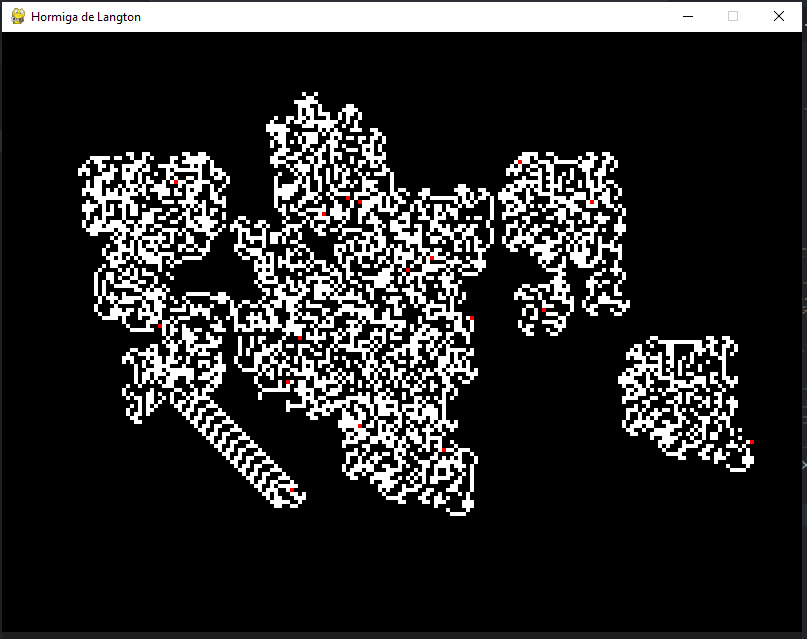
\includegraphics[keepaspectratio,alt={captura\_hormiga\_de\_langton.png}]{TP1_files/captura_hormiga_de_langton.png}}
\caption{captura\_hormiga\_de\_langton.png}
\end{figure}

    \subsubsection{\texorpdfstring{9. El Juego de la Vida de Conway consiste
en un tablero donde cada casilla representa una célula, de manera que a
cada célula le rodean 8 vecinas. Las células tienen dos estados: están
\emph{vivas} o \emph{muertas}. En cada iteración, el estado de todas las
células se tiene en cuenta para calcular el estado siguiente en
simultáneo de acuerdo a las siguientes
acciones:}{9. El Juego de la Vida de Conway consiste en un tablero donde cada casilla representa una célula, de manera que a cada célula le rodean 8 vecinas. Las células tienen dos estados: están vivas o muertas. En cada iteración, el estado de todas las células se tiene en cuenta para calcular el estado siguiente en simultáneo de acuerdo a las siguientes acciones:}}\label{el-juego-de-la-vida-de-conway-consiste-en-un-tablero-donde-cada-casilla-representa-una-cuxe9lula-de-manera-que-a-cada-cuxe9lula-le-rodean-8-vecinas.-las-cuxe9lulas-tienen-dos-estados-estuxe1n-vivas-o-muertas.-en-cada-iteraciuxf3n-el-estado-de-todas-las-cuxe9lulas-se-tiene-en-cuenta-para-calcular-el-estado-siguiente-en-simultuxe1neo-de-acuerdo-a-las-siguientes-acciones}

\begin{itemize}
\item
  Nacer: Si una célula muerta tiene exactamente 3 células vecinas vivas,
  dicha célula pasa a estar viva.
\item
  Morir: Una célula viva puede morir sobrepoblación cuando tiene más de
  tres vecinos alrededor o por aislamiento si tiene solo un vecino o
  ninguno.
\item
  Vivir: una célula se mantiene viva si tiene 2 o 3 vecinos a su
  alrededor.

  Caracterice el agente con su tabla REAS y las propiedades del entorno
  para después programarlo en Python:
\end{itemize}

    \textbf{Análisis REAS} \textbar{} Sistema \textbar{} Rendimiento
\textbar{} Entorno \textbar{} Actuadores \textbar{} Sensores \textbar{}
\textbar---------\textbar-------------\textbar---------\textbar------------\textbar----------\textbar{}
\textbar{} Juego de la Vida de Conway \textbar{} Evolución correcta de
las células siguiendo las reglas de Nacer, Morir, Vivir en cada
intervalo de tiempo y representación de su estado en el tablero.
\textbar{} Tablero (matriz), casillas donde viven las células \textbar{}
Comandos para cambiar el estado de las células según las reglas,
mediante la funcion \emph{actualizar-grilla} \textbar{} Lectura del
estado actual del tablero: contabilidad del número de células vivas
alrededor de cada una, medinte la funcion \emph{contar-vecinos}
\textbar{}

\textbf{Propiedades del entorno} \textbar{} Propiedad \textbar{}
\textbar{} \textbar-----------\textbar--\textbar{} \textbar{}
Observabilidad \textbar{} Total. Se puede saber en todo momento qué
células están vivas y cuáles no. \textbar{} \textbar{}
Determinista/Estocástico \textbar{} Las células siempre cambian su
estado en base a las reglas. \textbar{} \textbar{} Episódico/Secuencial
\textbar{} Episódico. La célula modifica su estado en base a la cantidad
de vecinos en cada iteración. \textbar{} \textbar{} Estatico/Dinamico
\textbar{} Estatico. La configuración de las células cambia de iteración
a iteración, pero no hay modificaciones intermedias que influyan en el
poder de decision de evolucion de la célula. \textbar{} \textbar{}
Discreto/Continuo \textbar{} Discreto en la práctica. La cantidad de
células representadas es un número finito. \textbar{} \textbar{} Agente
\textbar{} Multiagente. La cantidad de células vivas influye en la
condición de vida de las otras. \textbar{}

\begin{figure}
\centering
\pandocbounded{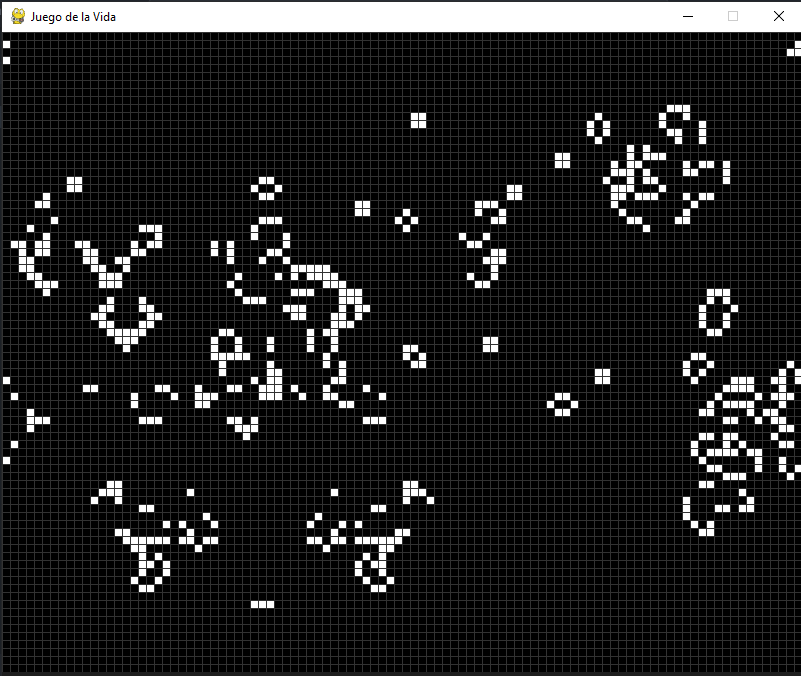
\includegraphics[keepaspectratio,alt={captura\_juego\_de\_la\_vida.png}]{TP1_files/captura_juego_de_la_vida.png}}
\caption{captura\_juego\_de\_la\_vida.png}
\end{figure}

    \section{Bibliografía}\label{bibliografuxeda}

\href{https://www.academia.edu/8241613/Inteligencia_Aritificial_Un_Enfoque_Moderno_2da_Edici\%C3\%B3n_Stuart_J_Russell_y_Peter_Norvig}{Russell,
S. \& Norvig, P. (2004) \emph{Inteligencia Artificial: Un Enfoque
Moderno}. Pearson Educación S.A. (2a Ed.) Madrid, España}

\href{https://artint.info/3e/html/ArtInt3e.html}{Poole, D. \& Mackworth,
A. (2023) \emph{Artificial Intelligence: Foundations of Computational
Agents}. Cambridge University Press (3a Ed.) Vancouver, Canada}


    % Add a bibliography block to the postdoc
    
    
    
\end{document}
